\section{Analysis of Features 3 and 4}

\subsection*{Empirical Results}

To further evaluate the discriminative landscape of the dataset, we analyze the statistical metrics and spatial distribution of Features 3 and 4.

\textbf{Distributions and Overlap:}
Based on the histograms (\texttt{feature\_3\_histogram.png} and \texttt{feature\_4\_histogram.png}), the distributions for both the Genuine and Fake classes are strictly unimodal, each exhibiting a single, well-defined peak. Observing the scatter plot (\texttt{features\_3\_4\_scatter.jpg}), we see that the classes occupy distinct, opposite quadrants. While there is a margin of overlap in the center $(0,0)$ region, the two distributions are clearly separated along a diagonal axis.

\textbf{Statistical Metrics:}
The computed statistics perfectly reflect this diagonal separation and structural similarity:
\begin{itemize}
    \item \textbf{Means:} The means are highly distinct and perfectly inverted between the classes. For the Fake class, the centroid is located in the top-left quadrant at Feature 3 = $-0.6809$ and Feature 4 = $0.6708$. For the Genuine class, the centroid is mirrored into the bottom-right quadrant at Feature 3 = $0.6652$ and Feature 4 = $-0.6642$.
    \item \textbf{Variances:} In stark contrast to Features 1 and 2, the variances here are remarkably symmetric. The variance for the Fake class is $0.5500$ (Feature 3) and $0.5360$ (Feature 4), while the Genuine class exhibits nearly identical variances of $0.5489$ (Feature 3) and $0.5533$ (Feature 4).
\end{itemize}

\begin{figure}[H]
    \centering
    \begin{minipage}{0.48\textwidth}
        \centering
        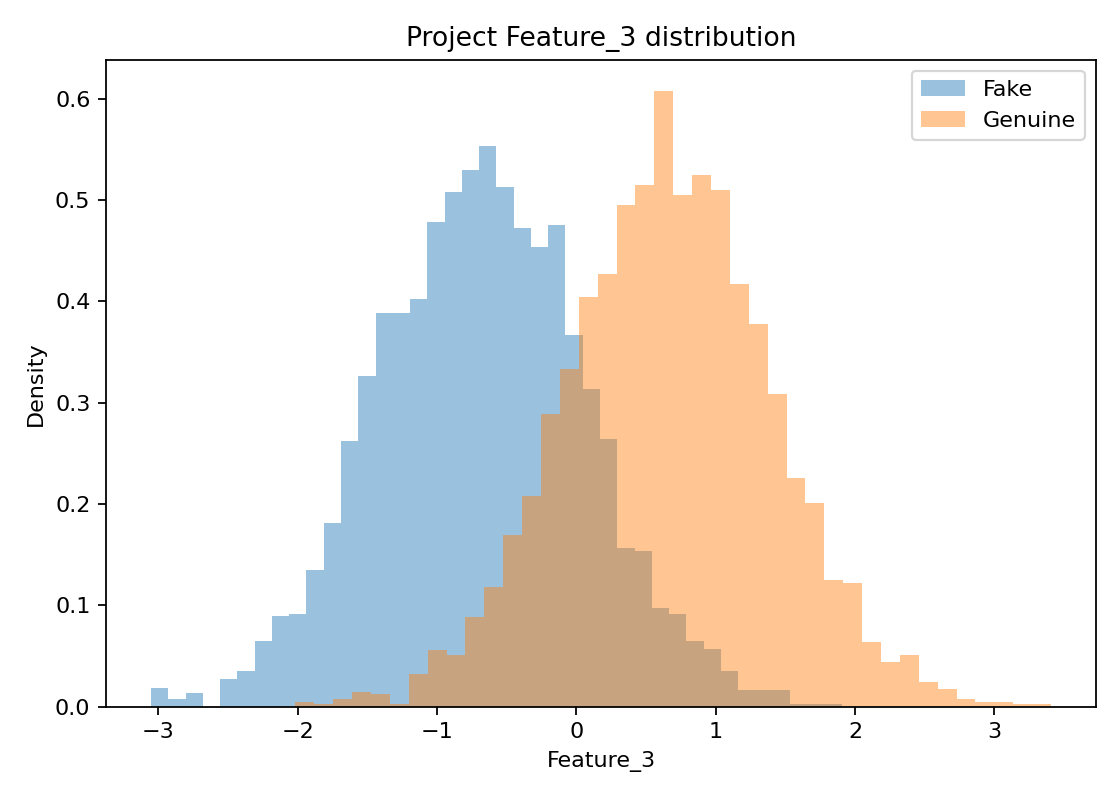
\includegraphics[width=\linewidth]{histograms/feature_3_histogram.png}
        \caption{Histogram of Feature 3.}
    \end{minipage}\hfill
    \begin{minipage}{0.48\textwidth}
        \centering
        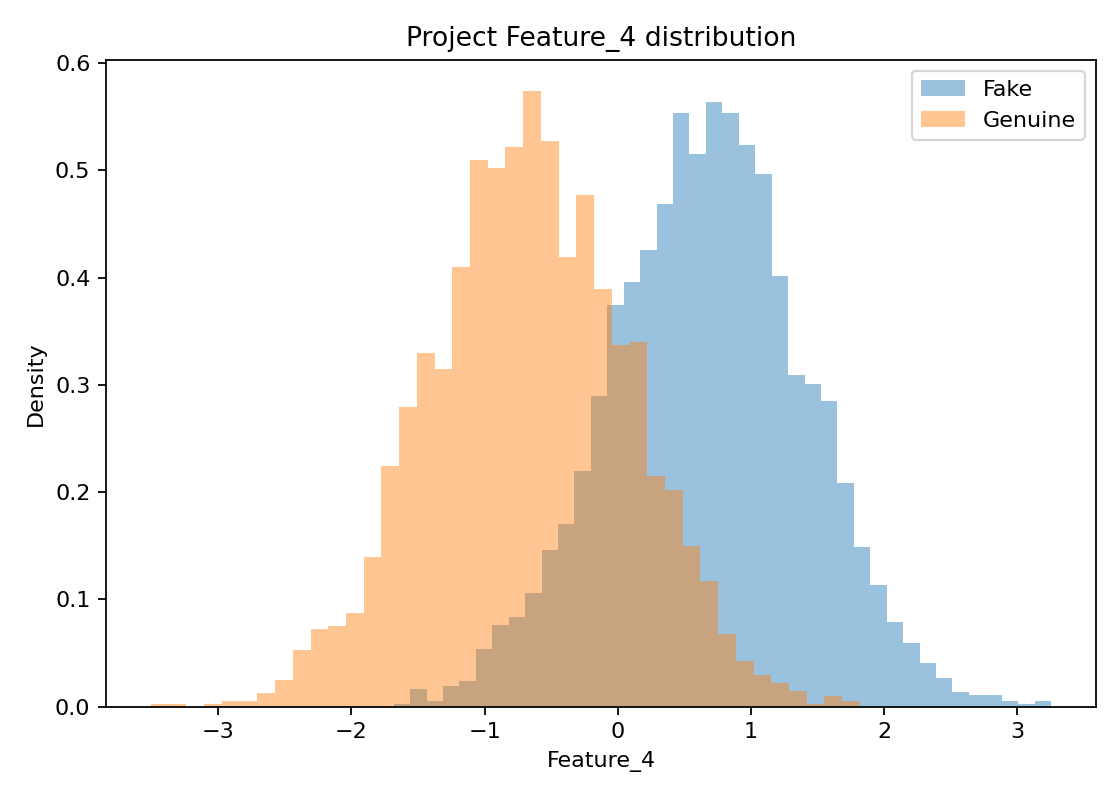
\includegraphics[width=\linewidth]{histograms/feature_4_histogram.png}
        \caption{Histogram of Feature 4.}
    \end{minipage}
\end{figure}

\begin{figure}[H]
    \centering
    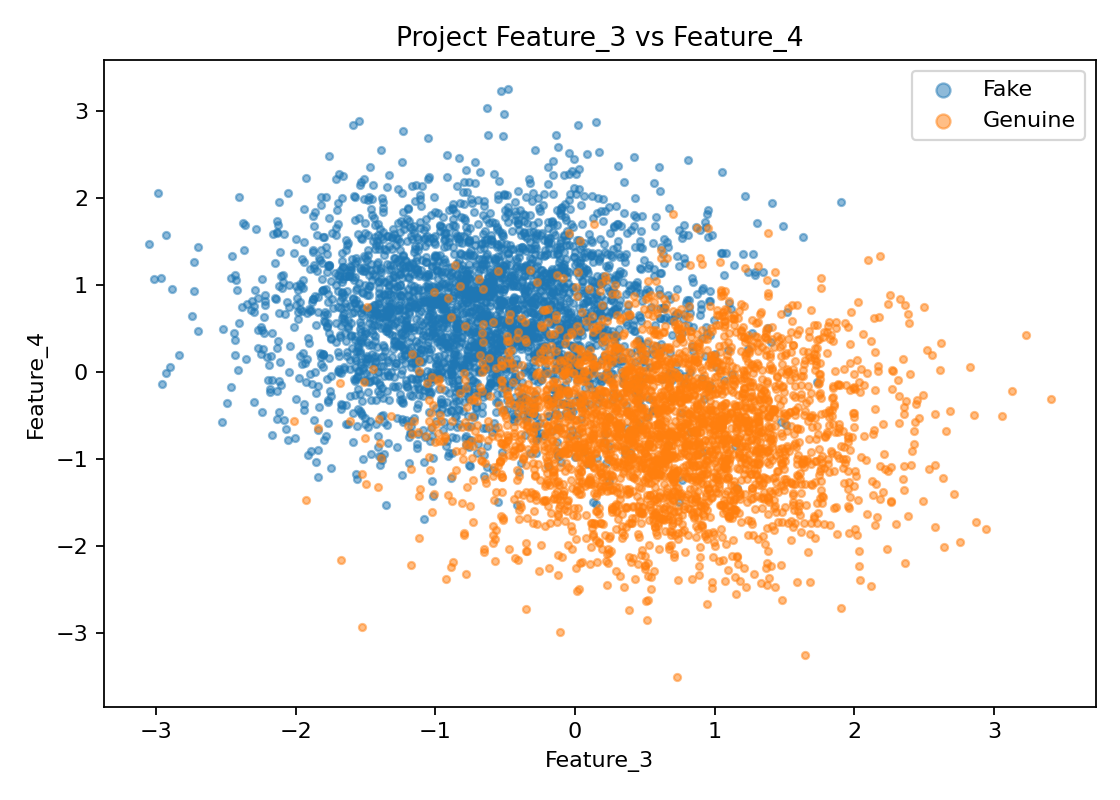
\includegraphics[width=0.6\textwidth]{scatters/features_3_4_scatter.png}
    \caption{Scatter plot of Feature 3 vs Feature 4, illustrating diagonal separation with symmetric class variances.}
    \label{fig:scatter_3_4}
\end{figure}

\subsection*{Theoretical Analysis}

The geometry of Features 3 and 4 represents a "textbook" Gaussian distribution scenario. Because both classes share virtually identical variances across both axes (approximately $\sim 0.54$), their scatter clusters have the exact same geometric "shape"—they are symmetric, roughly spherical clouds of data.

Because their shapes are identical, the classes differentiate themselves entirely through a spatial shift (the translation of their means). The Fake class is shifted to the top-left, and the Genuine class is shifted to the bottom-right, creating the most linearly separable feature pair in the entire dataset.

\subsection*{Motivation and Future Insights}

The "well-behaved" nature of Features 3 and 4 provides a critical counterpoint to the chaotic topology of the other features, offering the following modeling insights:

\begin{enumerate}
    \item \textbf{Suitability for Linear Models:} Because the classes have identical covariance spreads and are separated by a spatial shift, a simple linear decision boundary (such as one generated by Logistic Regression or Linear Discriminant Analysis) would be highly effective if these were the only two features in the dataset. A straight diagonal line cleanly bisecting the space between the centroids would achieve a low error rate.
    \item \textbf{The Tied MVG Trap:} Features 3 and 4 are the only features where the fundamental assumption of the Tied Covariance MVG actually holds true. The Tied MVG assumes that all classes share the exact same covariance matrix. While this assumption is valid for Features 3 and 4, applying it to the entire 6-dimensional dataset forcefully averages the inverted variances of Features 1/2 and destroys the multi-modal clusters of Features 5/6, which explains the catastrophic calibration loss the Tied model suffered in Laboratory 10. 
\end{enumerate}